% Préambule commun des schémas TikZ (compilés séparément par construire_figures.py)
\documentclass[tikz,border=3pt]{standalone}
\usepackage[T1]{fontenc}
\usepackage[utf8]{inputenc}
\usepackage{lmodern}
\usepackage{amsmath,amssymb}
\usepackage{bm}
\usepackage[american,siunitx,straightvoltages]{circuitikz}
\usetikzlibrary{arrows.meta,positioning,calc,decorations.pathmorphing,
  decorations.markings,decorations.pathreplacing,patterns,shapes.geometric,
  shapes.misc,shapes.multipart,fit,backgrounds,3d,intersections,matrix}

\ctikzset{bipoles/length=1.1cm, amplifiers/scale=0.85, tripoles/op amp/width=1.4}

\tikzset{
  >={Latex[length=2mm,width=1.4mm]},
  every picture/.style={line width=0.6pt, font=\small},
  % schémas-blocs
  bloc/.style={draw, minimum width=1.5cm, minimum height=0.9cm, align=center,
               inner sep=3pt, fill=white},
  somme/.style={draw, circle, minimum size=4.5mm, inner sep=0pt, fill=white,
                path picture={\draw (path picture bounding box.north west)
                  -- (path picture bounding box.south east)
                  (path picture bounding box.north east)
                  -- (path picture bounding box.south west);}},
  gain/.style={draw, isosceles triangle, isosceles triangle apex angle=60,
               minimum size=8mm, inner sep=1pt, fill=white},
  bruit/.style={draw, circle, minimum size=4.5mm, inner sep=0pt, fill=white,
                path picture={\node at (path picture bounding box.center)
                  {\scriptsize$\ast$};}},
  cadre/.style={draw, dashed, rounded corners=1pt},
  cadrept/.style={draw, dash dot, rounded corners=1pt},
  fleche/.style={->},
  % mécanique
  bati/.style={pattern=north east lines, draw=none},
  ressort/.style={decorate, decoration={coil, aspect=0.4, segment length=2.2mm,
                  amplitude=2mm, pre length=2mm, post length=2mm}},
  zigzag/.style={decorate, decoration={zigzag, segment length=2mm,
                  amplitude=1.6mm, pre length=2mm, post length=2mm}},
  pivot/.style={draw, circle, fill=white, minimum size=2.2mm, inner sep=0pt},
  masse/.style={draw, fill=gray!25, minimum width=1.4cm, minimum height=0.8cm},
  cote/.style={<->, line width=0.4pt},
  axe/.style={->, line width=0.6pt},
  trait mixte/.style={dash dot, line width=0.4pt},
}

% Encastrement / bâti hachuré : \bati{(x1,y1)}{(x2,y2)} trace une ligne et ses hachures dessous
\newcommand{\bati}[3][0.18]{%
  \fill[pattern=north east lines] #2 rectangle ($#3+(0,-#1)$);
  \draw[line width=0.8pt] #2 -- #3;}

% Transducteur (deux cercles entrelacés) : \pic (t) at (x,y) {transducteur};  -> (t-o) entrée, (t-e) sortie
\tikzset{
  transducteur/.pic={\draw (-0.13,0) circle (0.24); \draw (0.13,0) circle (0.24);
    \coordinate (-o) at (-0.37,0); \coordinate (-e) at (0.37,0);
    \coordinate (-n) at (0,0.24); \coordinate (-s) at (0,-0.24);},
  bobine/.style={decorate, decoration={coil, aspect=0.7, segment length=1.4mm,
                 amplitude=1.6mm, pre length=1mm, post length=1mm}},
  sourcebruit/.style={draw, circle, minimum size=5mm, inner sep=0pt, fill=white,
                 label={[inner sep=0pt]center:$\ast$}},
  sourcecourant/.style={draw, circle, minimum size=5mm, inner sep=0pt, fill=white,
                 label={[inner sep=0pt]center:$\circledast$}},
}

% Composants compacts (pour les petits boîtiers des schémas-blocs)
\newcommand{\resistance}[2]{% de #1 à #2 (quelconque)
  \draw #1 -- ($#1!0.22!#2$) ($#1!0.78!#2$) -- #2;
  \draw[decorate, decoration={zigzag, segment length=1.5mm, amplitude=1.1mm}]
    ($#1!0.22!#2$) -- ($#1!0.78!#2$);}
\newcommand{\condensateur}[2]{% horizontal de #1 à #2
  \draw #1 -- ($($#1!0.5!#2$)+(-0.05,0)$) ($($#1!0.5!#2$)+(0.05,0)$) -- #2;
  \draw[line width=1pt] ($($#1!0.5!#2$)+(-0.05,0.14)$) -- ($($#1!0.5!#2$)+(-0.05,-0.14)$)
                        ($($#1!0.5!#2$)+(0.05,0.14)$) -- ($($#1!0.5!#2$)+(0.05,-0.14)$);}
% R // C horizontal : \RparC{(x,y)}{longueur}{écart}  (centre, longueur totale, écart vertical)
\newcommand{\RparC}[3]{%
  \coordinate (rcA) at ($#1+(-#2/2,0)$); \coordinate (rcB) at ($#1+(#2/2,0)$);
  \draw (rcA) -- ++(0.15,0) coordinate (rcA1) (rcB) -- ++(-0.15,0) coordinate (rcB1);
  \draw (rcA1) -- ++(0,#3/2) (rcA1) -- ++(0,-#3/2) (rcB1) -- ++(0,#3/2) (rcB1) -- ++(0,-#3/2);
  \resistance{($(rcA1)+(0,#3/2)$)}{($(rcB1)+(0,#3/2)$)}
  \condensateur{($(rcA1)+(0,-#3/2)$)}{($(rcB1)+(0,-#3/2)$)}}

\newcommand{\creneau}[3]{% origine, suite de niveaux (pas 0.3), étiquette
  \begin{scope}[shift={#1}]
    \def\x{0}\def\prev{0}
    \foreach \y [count=\i] in {#2} {
      \pgfmathsetmacro{\xa}{(\i-1)*0.3}\pgfmathsetmacro{\xb}{\i*0.3}
      \draw (\xa,\y*0.4) -- (\xb,\y*0.4);
      \ifnum\i>1 \pgfmathsetmacro{\yp}{\prevy}\draw (\xa,\yp*0.4) -- (\xa,\y*0.4); \fi
      \xdef\prevy{\y}}
    \node[left, font=\footnotesize] at (-0.1,0) {#3};
  \end{scope}}
\begin{document}
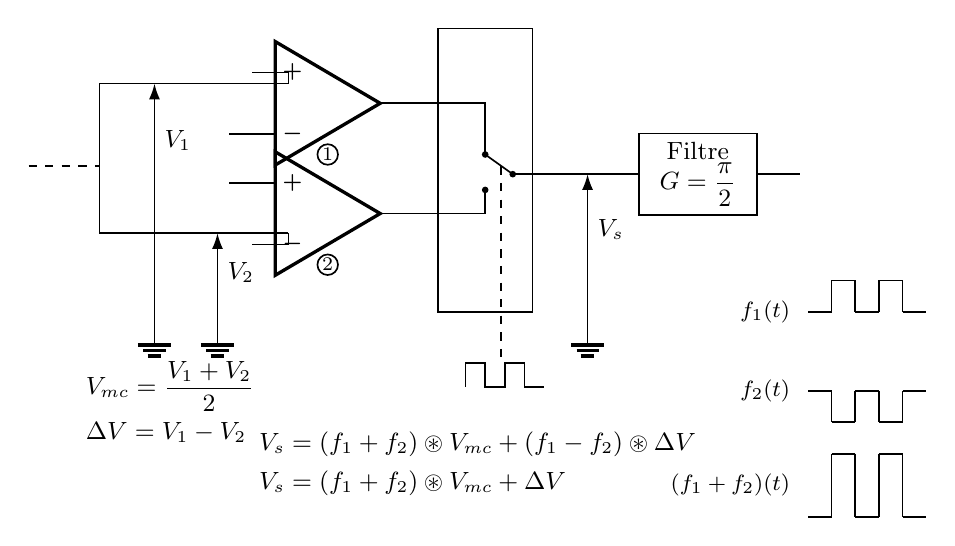
\begin{tikzpicture}[font=\small]
  \draw[dashed] (-1.2,0.85) -- (-0.3,0.85);
  \draw (-0.3,1.9) -- (2.1,1.9) (-0.3,0) -- (2.1,0) (-0.3,1.9) -- (-0.3,0);
  \draw (2.6,1.65) node[op amp, noinv input up, scale=0.8] (a1) {};
  \draw (2.6,0.25) node[op amp, noinv input up, scale=0.8] (a2) {};
  \node[draw, circle, inner sep=0.5pt, font=\scriptsize] at (2.6,1.0) {1};
  \node[draw, circle, inner sep=0.5pt, font=\scriptsize] at (2.6,-0.4) {2};
  \draw (2.1,1.9) |- (a1.+); \draw (2.1,0) |- (a2.-);
  \draw (a1.-) -- ++(-0.3,0); \draw (a2.+) -- ++(-0.3,0);
  \draw[->] (0.4,-1.0) -- (0.4,1.9) node[pos=0.75, right] {$V_1$};
  \draw[->] (1.2,-1.0) -- (1.2,0) node[pos=0.5, right] {$V_2$};
  \draw (0.4,-1.0) node[ground] {} (1.2,-1.0) node[ground] {};
  % commutateur
  \draw (4.0,-1.0) rectangle (5.2,2.6);
  \draw (a1.out) -- (4.6,1.65) -- (4.6,1.0); \fill (4.6,1.0) circle (1.2pt);
  \draw (a2.out) -- (4.6,0.25) -- (4.6,0.55); \fill (4.6,0.55) circle (1.2pt);
  \draw (4.6,1.0) -- (4.95,0.75); \fill (4.95,0.75) circle (1.2pt);
  \draw[dashed] (4.8,0.85) -- (4.8,-1.6);
  \draw (4.35,-1.95) -- (4.35,-1.65) -- (4.6,-1.65) -- (4.6,-1.95) -- (4.85,-1.95) -- (4.85,-1.65) -- (5.1,-1.65) -- (5.1,-1.95) -- (5.35,-1.95);
  \draw (4.95,0.75) -- (6.6,0.75);
  \draw[->] (5.9,-1.0) -- (5.9,0.75) node[pos=0.6, right] {$V_s$}; \draw (5.9,-1.0) node[ground] {};
  \node[bloc, align=center] (f) at (7.3,0.75) {Filtre\\$G = \dfrac{\pi}{2}$};
  \draw (f.east) -- (8.6,0.75);
  % relations
  \node[align=left, anchor=north west] at (-0.6,-1.5) {$V_{mc} = \dfrac{V_1+V_2}{2}$\\[3pt]$\Delta V = V_1 - V_2$};
  \node[align=left, anchor=north west] at (1.6,-2.4) {$V_s = (f_1+f_2)\circledast V_{mc} + (f_1-f_2)\circledast\Delta V$\\[3pt]$V_s = (f_1+f_2)\circledast V_{mc} + \Delta V$};
  % créneaux
  \creneau{(8.7,-1.0)}{0,1,0,1,0}{$f_1(t)$}
  
  \creneau{(8.7,-2.0)}{0,-1,0,-1,0}{$f_2(t)$}
  
  \creneau{(8.7,-3.2)}{-1,1,-1,1,-1}{$(f_1+f_2)(t)$}
\end{tikzpicture}
\end{document}
